\section{\label{sec:scale}Scaling Analysis}
The Gung Ho dynamical core uses an unstructured mesh to avoid a
singular pole which ultimately inhibits the scaling of the
UM. Examining the scaling behavour of the model to if the model can
perform sufficiently well is important. To test the scaling a series
of model runs was performed. The version of the LFRic repository trunk
was $17483$. The code was compiled on the XCS with the Intel 17
compiler, at production level which is \verb+-O3+. The baroclinic wave
test was run on a $C576$ mesh with 30 levels. The time-step was $180$s
seconds and the benchmarks were run for $100$ time-steps. The code was
profiled using the CrayPAT tool in sampling mode. 

\begin{figure}
\centering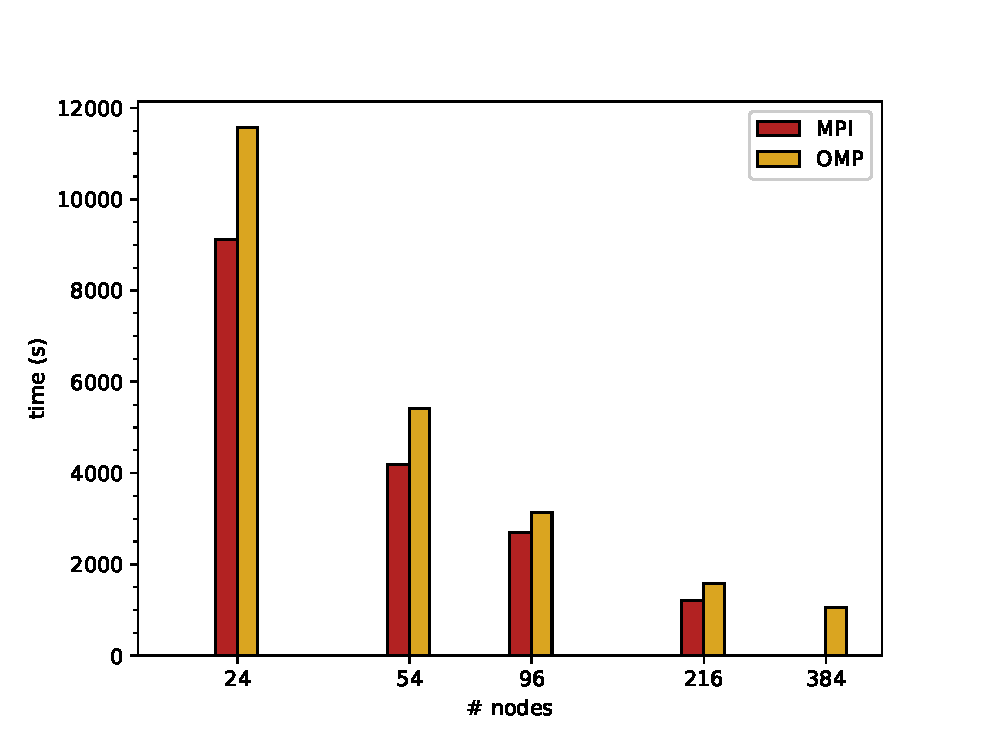
\includegraphics[width=1.0\linewidth]{figs/wc-scale.eps}
\caption{\label{fig:wc_scale}Wall-clock time strong scaling of the 
  Baroclinic wave test.}
\end{figure} 

\begin{figure}
\centering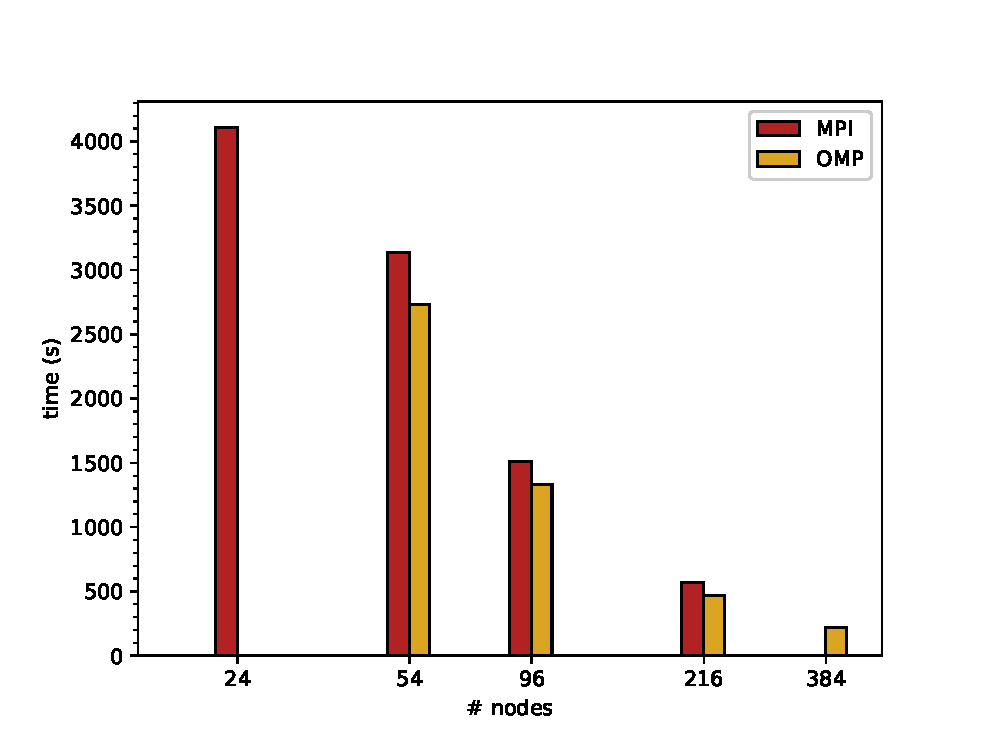
\includegraphics[width=1.0\linewidth]{figs/U-scale.eps}
\caption{\label{fig:U_scale}Wall-clock time strong scaling of the 
  User code from Baroclinic wave test.}
\end{figure} 

\begin{figure}
\centering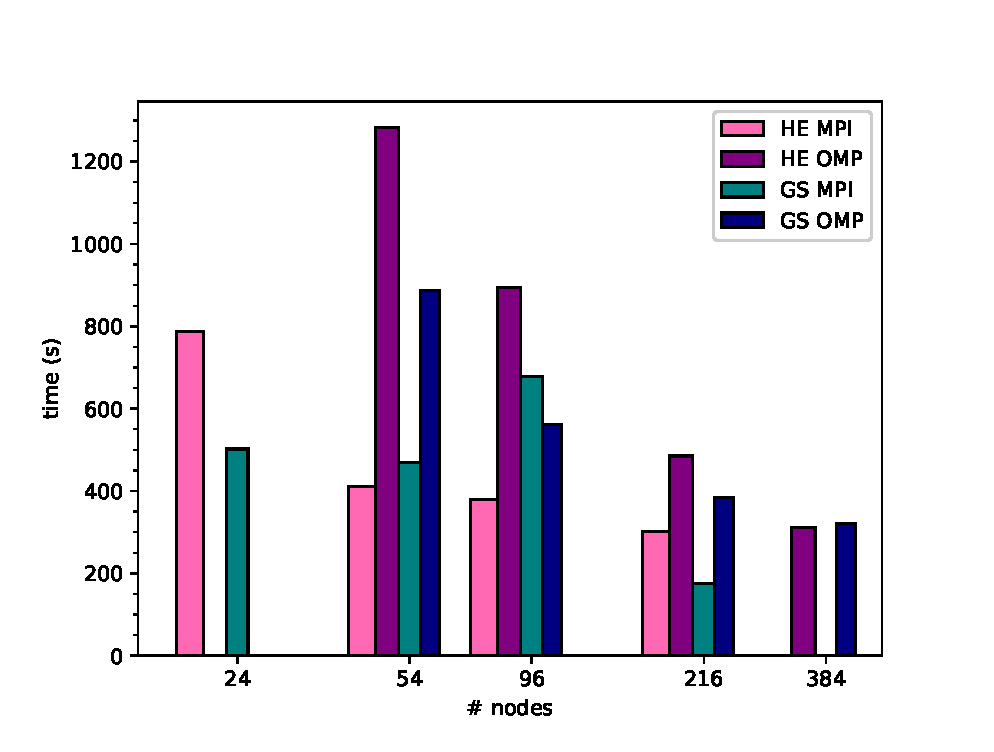
\includegraphics[width=1.0\linewidth]{figs/comms-scale.eps}
\caption{\label{fig:comns_scale}Wall-clock time strong scaling of the 
  communications costs of the Baroclinic wave test.}
\end{figure} 

Shown in figure~\ref{fig:wc_scale} is the strong scaling 